\documentclass[nynorsk,12pt,a4paper]{article}
\usepackage[utf8]{inputenc}
\usepackage[T1]{fontenc}
\usepackage{graphicx}
\usepackage{babel}
\renewcommand*{\familydefault}{\rmdefault}
\title{Arkitekturdokument\\
Dynamisk Nettverksbrannmur
}
\author{Espen Gjærde \and Svein Ove Undal}
\date{11.04.2013}

\pagenumbering{arabic}
\begin{document}
\maketitle
\newpage

\section*{Revisjonshistorie}

\begin{table}[h!]
	\begin{tabular}{ l l l l }

		\textsc{Dato} & \textsc{Versjon} & \textsc{Forklaring} & \textsc{Forfattar} \\
		\hline 
		15.04.2013 & 1.0 & Dokumentet oppretta & Espen \\ 
		16.04.2013 & 1.0 & Diagram og illustrasjonar oppdatert & Espen \\
		\hline
	\end{tabular}
\end{table}

\newpage
\tableofcontents{}

\newpage

\section{Innleiing}
\subsection{Hensikta med dokumentet}
Dette dokumentet skal beskrive arkitekturen i systemet som blir utvikla. Dokumentet vil gå djupare inn i dei forskjellige systema som vert nytta og korleis desse heng saman. Også her vert det nytta standardiserte logiske modellar for å gje ei betre oversikt over systemet.

\subsection{Avgrensingar}
Dokumentet skildrar systemet som vert utvikla, og relasjonar til andre system. Det vil ikkje skildre eksterne system som vert nytta.

\subsection{Definisjonar og forkortingar}
\begin{table}[h!]
	\begin{tabular}{ l p{11cm} }
	\textsc{Ord} & \textsc{Forklaring / Definisjon} \\ \hline
	IPtables & Pakkefilter /-manipulator tilgjengeleg i dei fleste linuxdistribusjonar \\
	Linux-distibusjon & Variant av operativsystemet linux \\
	WebUI & Nettside som kontrollerer eit system/program. \\
	DNF	& Systemet som vert utvikla (\emph{Eng: Dynamic Network Firewall}) \\
	Ruting & Sending/Vidaresending av pakkar i eit nettverk \\
	Prerouting & (\emph{Nor: Før-ruting}) behandling av pakkar før dei blir ruta \\
	Daemon & Program som kjører i bakgrunn og utfører oppgaver automatisk. \\
	\hline
	\end{tabular}
\end{table}

%\subsection{Referansar}
\subsection{Oversikt over innhald}
\paragraph{}
Dette dokumentet er av litt meir teknisk art, og inneheld ein modellar for å forklare korleis komponentane i systemet heng saman, og korleis dei kommuniserer med andre komponentar i operativsystemet. Her vil være både UML-standardmodellar, og figurar som bryt noko med UML-standarden. Figurar som bryt litt med standarden vil verte forklart nærmare.

\newpage
\section{Bakgrunn og oversikt}
\subsection{UseCase modell}
UseCase-modellen i figur 1 gir eit bilete av kva funksjonar brukarane av systemet skal ha tilgjeneleg.
\begin{figure}[h!]
	\includegraphics[scale=0.5]{imgs/UC.eps}
	\caption{UseCase-modell}
\end{figure}

\subsection{Ikkje-funksjonelle krav}
Systemet vert utvikla under ein open lisens, og skal være tilgjengeleg for allmennheita. Det vil ikkje følgje nokon garantiar eller krav til service og støtte til systemet. 
\subsection{Vilkår og avhengigheiter}
\paragraph{Tjenarside}
Systemet vert utviklar for Debian Linux, og er avhengig av programmeringsspråket Python, brannmursystemet Iptables og Linux Traffic Control. Alle desse skal være implementert i dei fleste linux-distribusjonar. Vi har også programmert systemet mot ein mySQL-database, men systemet sine grunnfunksjonar kan fungere utan databasen. For authentisering vert linux sitt PAM-system nytta.
\paragraph{Klientside}
Systemet nyttar webteknologi for å authentisere klientar opp mot systemet. Klientar som skal nytte systemet må derfor ha ein nettlesar. Vi anbefala ein nettlesar av nyare dato.
 
\newpage
\section{Arkitekturperspektiv}
\subsection{Logisk}
\begin{figure}[h!]
	\centering
	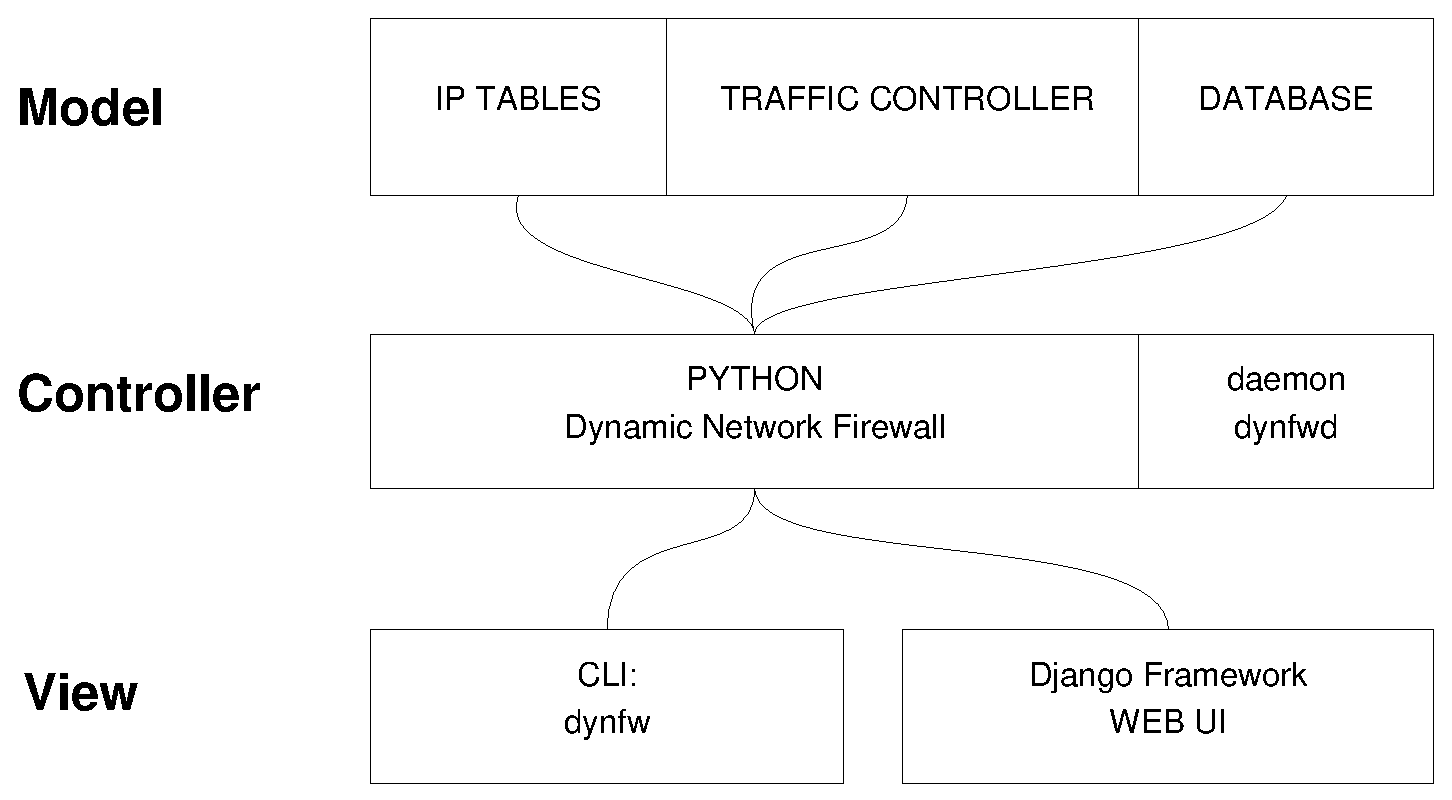
\includegraphics[scale=0.5]{imgs/logisk.eps}
	\caption{MVC-oppsett av systemet.}
	\label{fig:MVC}
\end{figure}

\newpage
\subsection{Prosess}
\subsubsection{Dynfw daemon}
\paragraph{Dynfwd} er ein tjeneste (deamon) som kjører i bakgrunnen og automatisk justerer brannmuren og vurderer om nokon av brukarane må avgrensast.
\begin{figure}[h!]
	\centering
	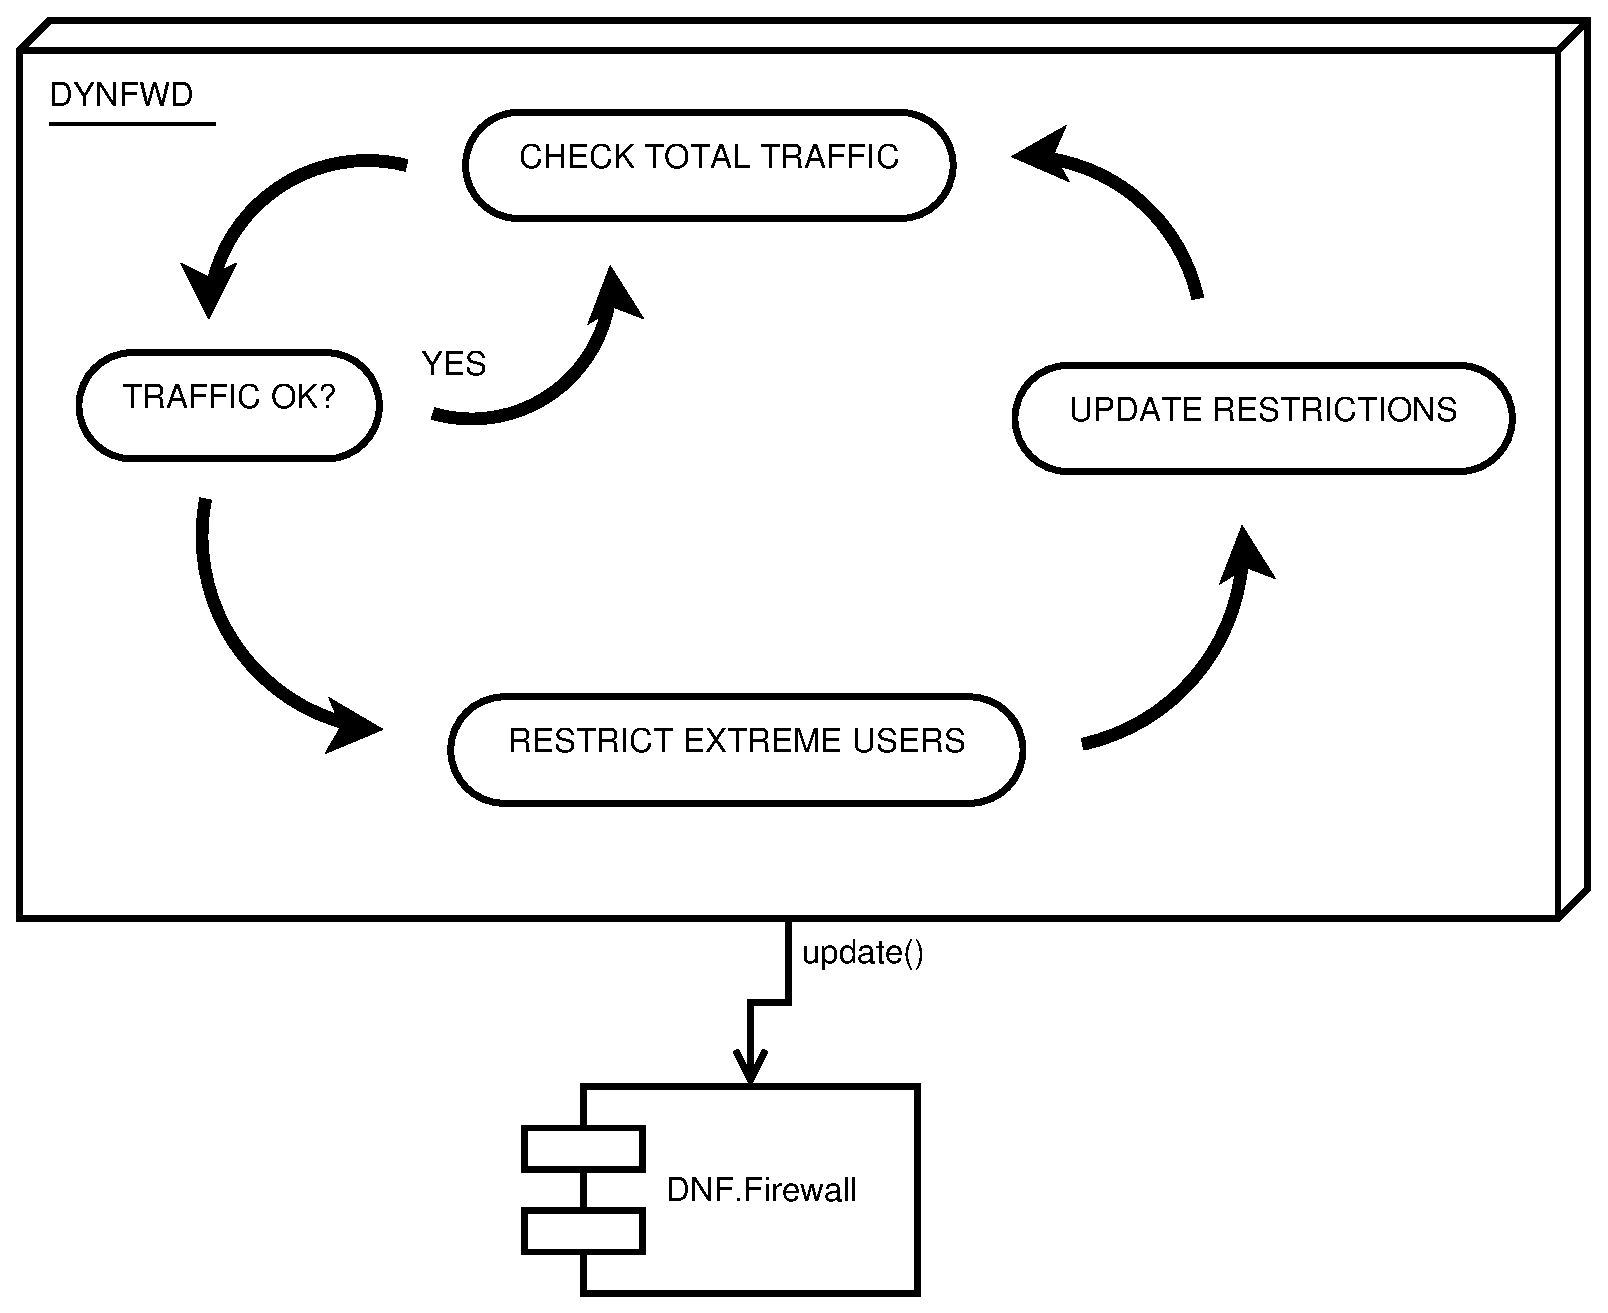
\includegraphics[scale=0.5]{imgs/dyndw.eps}
	\caption{grov skisse over dynfwd si framferd}
	\label{fig:dynfw}
\end{figure}

\newpage
\subsection{Implemetasjon}
\paragraph{}
Vi kan seie at systemet har tre hovuddelar (sjå også figur \ref{fig:MVC}). Figur \ref{fig:impl} viser korleis programmvara vi har koda snakkar med dei andre komponentane når nokon nyttar webgrensesnittet. Det gir også ei oversikt over kva pakkar som har ansvar for dei forskjellige linux-komponentane som systemet samarbeider med. Det er verd å merke seg at den automatiske justeringa ikkje kjem til syne i figur 3.
\begin{figure}[h!]
	\centering
	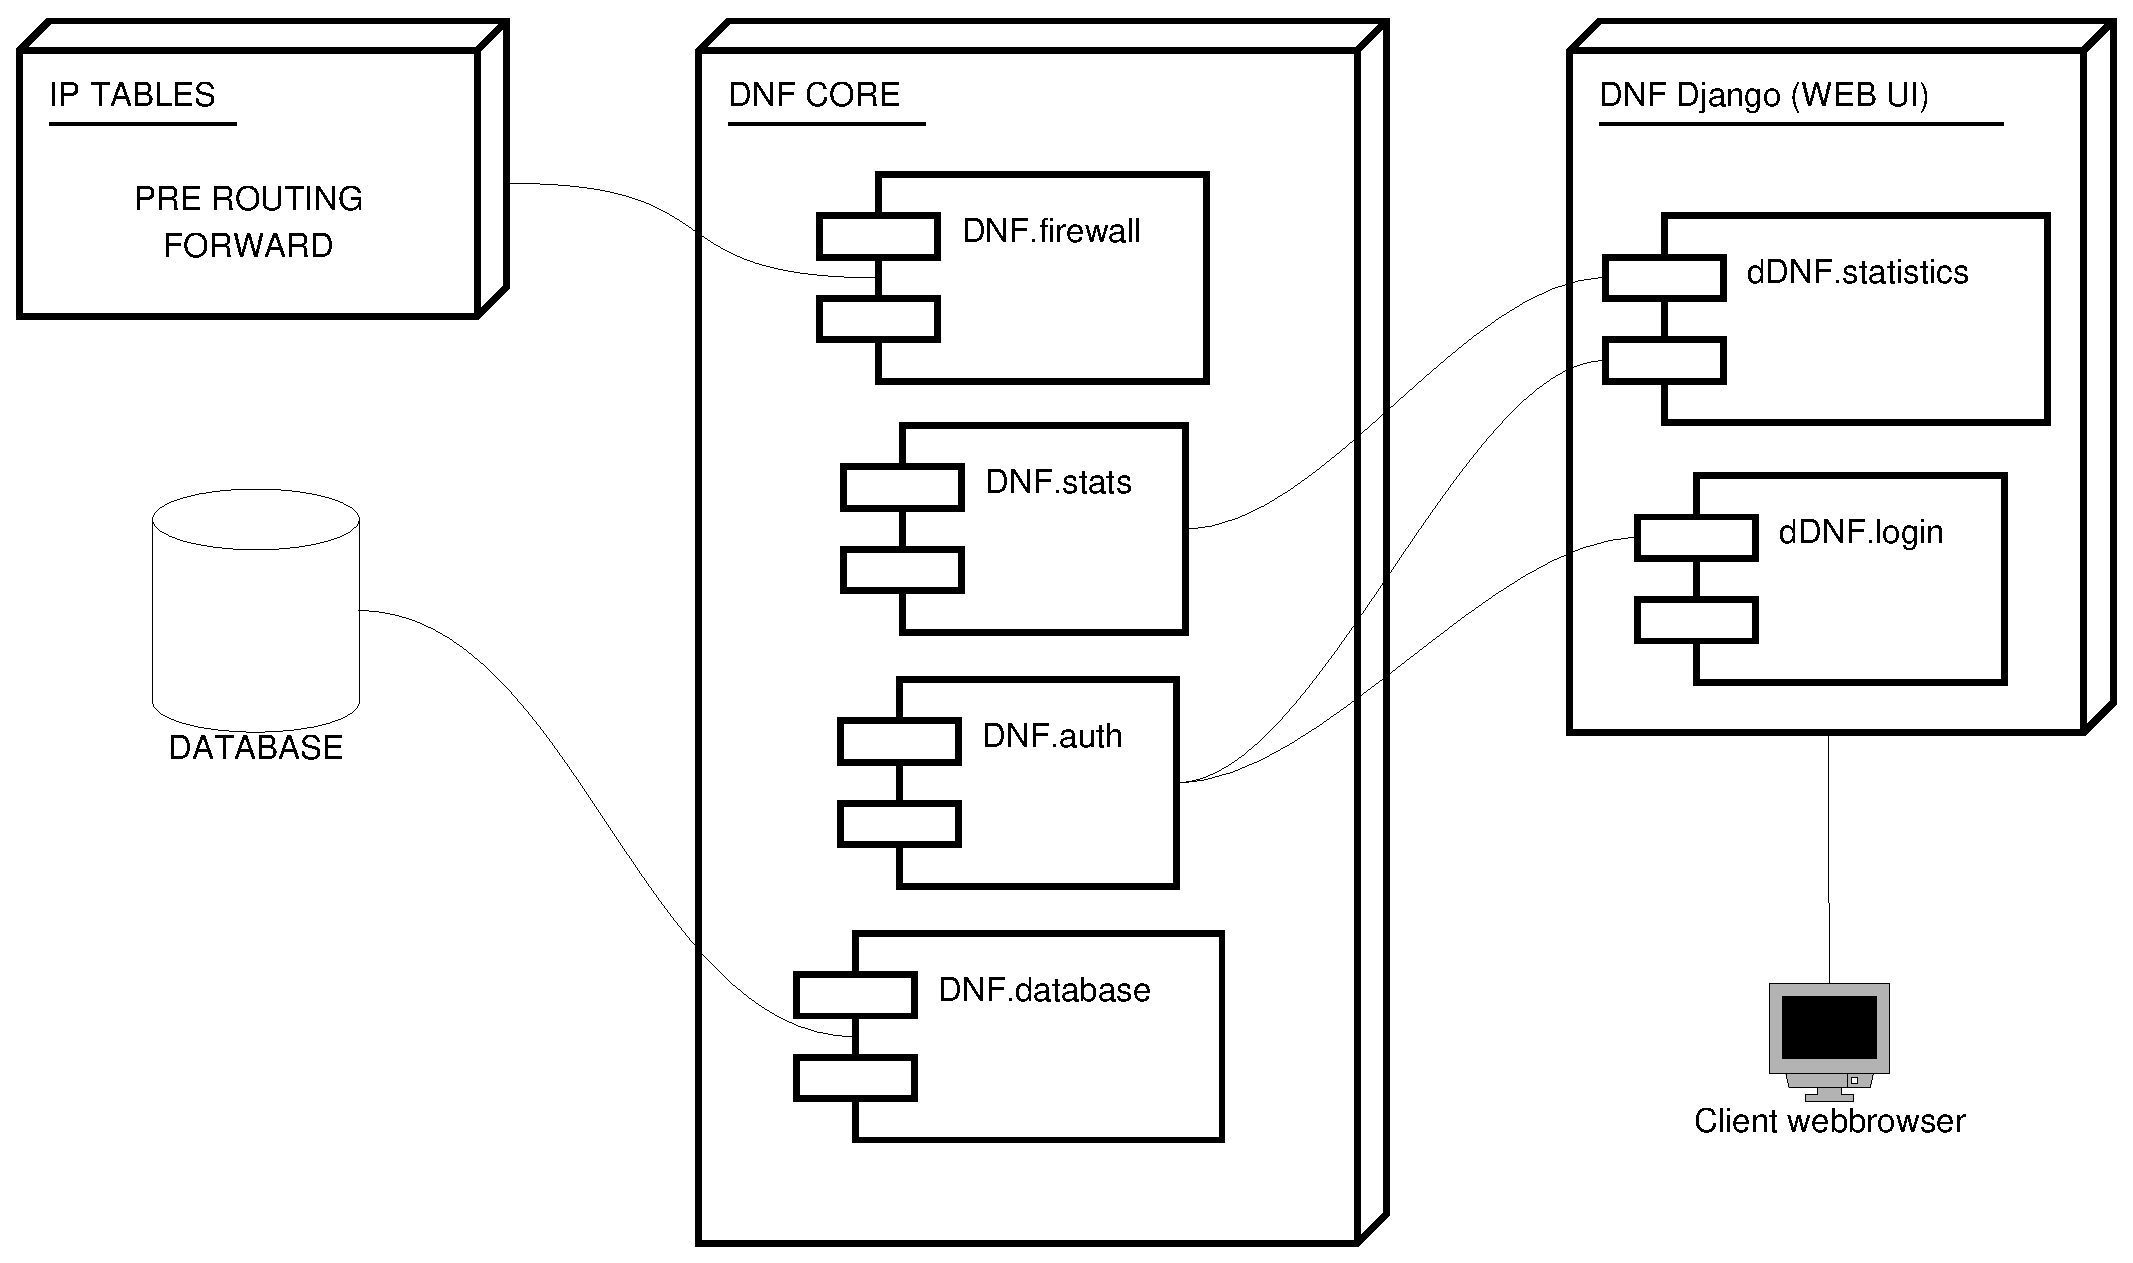
\includegraphics[scale=0.45]{imgs/implementasjon.eps}	
	\caption{Implementasjonsperspektivet}
	\label{fig:impl}
\end{figure}

\newpage
\subsection{Andre perspektiv}
\subsubsection{Nettverksbehandling}
Figur \ref{fig:iptables} viser korleis trafikken blir behandla internt i systemet. Trafikken går først til linux si mekanisme <<Traffic Control>>, der pakkar som bryt med eit gitt regelverk blir merka. Pakkar går så vidare inn i førruting-regelsettet i Iptables. Her blir det sjekka om ipadressa alt er registrert og logga inn. Om ipadressa ikkje er logga inn, blir trafikken fanga opp og omruta til ei påloggingside.
Trafikken blir deretter sendt gjennom ei regelsettet for vidaresending, der det blir sjekka om nokon er svartelista, om trafikken er merka og om personen framleis er pålogga og aktiv. 
\begin{figure}[h!]
\paragraph{Nettverksflyt internt}
	\centering
	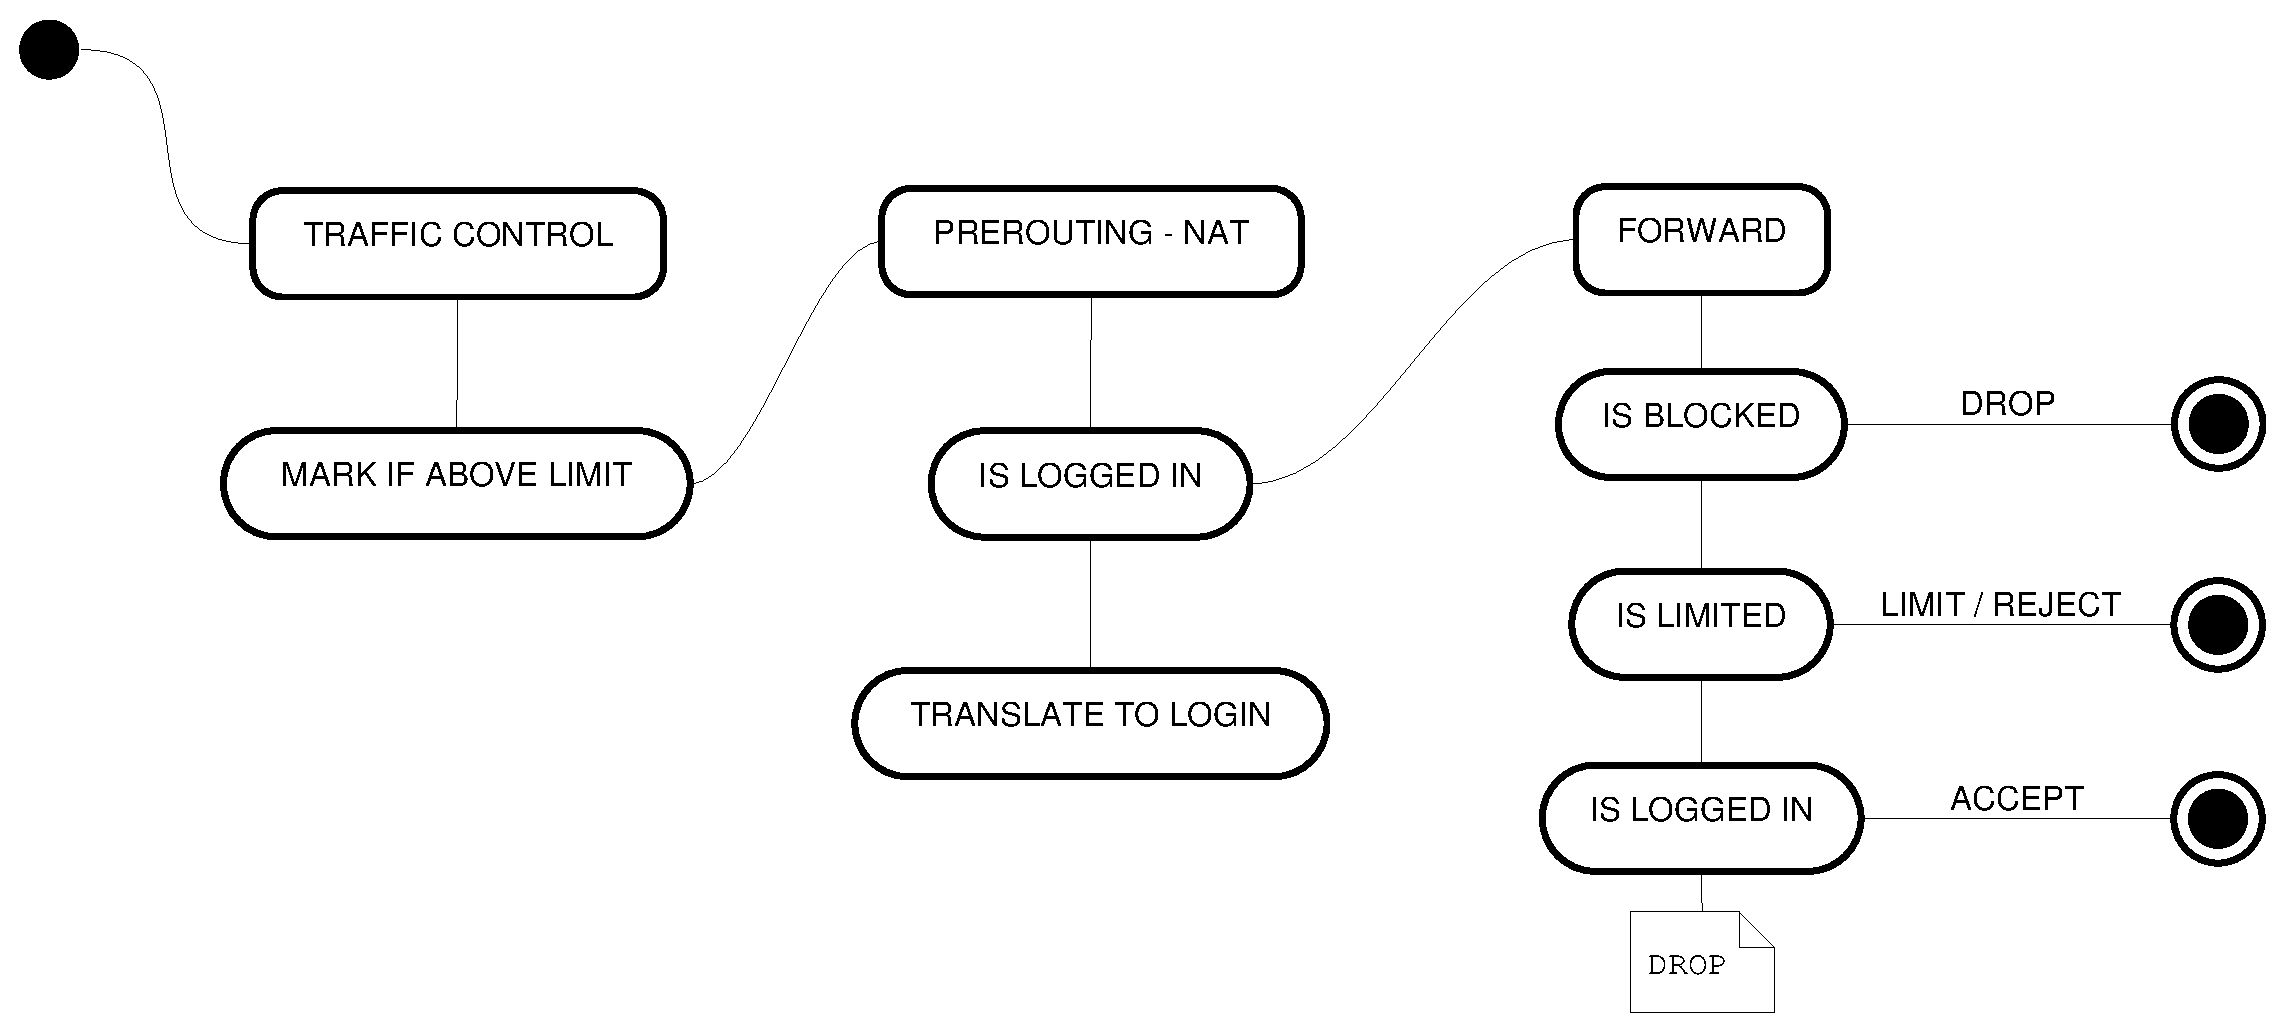
\includegraphics[scale=0.45]{imgs/iptables.eps}
	\caption{Skisse over flyt gjennom brannmur}
	\label{fig:iptables}
\end{figure}
\newpage
\subsubsection{Systemet si plassering i nettverket}
Nettverkskissa i figur \ref{fig:nett} viser korleis nettverket \emph{kan} settast opp. Det er ikkje naudsynt med ein ekstern brukardatabase, sjølv om det vil være naturleg å ha. Det er også fullt mogleg å ha all rutingfunksjon i same system som dette systemet.
\begin{figure}[h!]
\paragraph{Nettverkskisse}
	\centering
	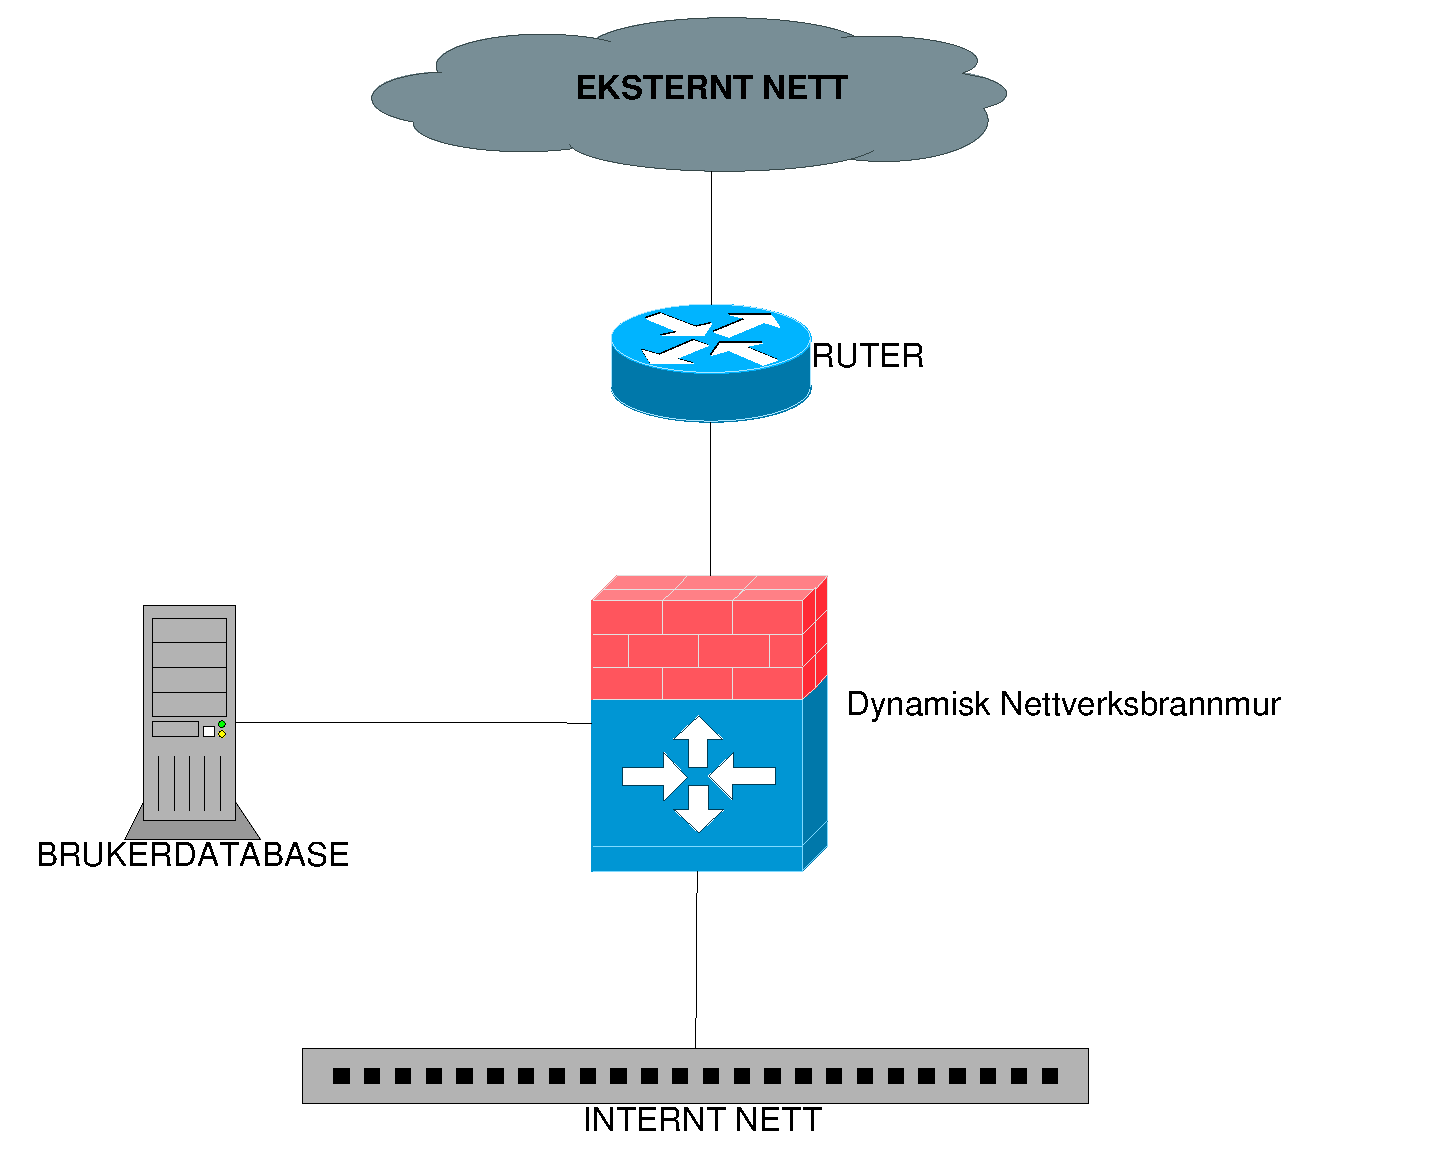
\includegraphics[scale=0.5]{imgs/nettverk.eps}
	\caption{Nettverkskisse}
	\label{fig:nett}
\end{figure}

%\section{Vedlegg}

\end{document}